% Full instructions available at:
% https://github.com/elauksap/focus-beamertheme

\documentclass[9pt]{beamer}
\usetheme{focus}

%%%%%%%%%%%%%%%%%%%%%%%%%%%%%%%%%%%%%%%%%%%%%%%%%%%%%%%%%%%%%%%%%%%%%
% Typography, change document font
\usepackage[tt=false, type1=true]{libertine}
\usepackage[varqu]{zi4}
\usepackage[libertine]{newtxmath}
\usepackage[T1]{fontenc}

\usepackage[protrusion=true,expansion=true]{microtype}

% Disable paragraph indentation, and increase gap
\usepackage{parskip}

%Matrix
\usepackage{tabstackengine}
\setstackEOL{;}% row separator
\setstackTAB{,}% column separator
\setstacktabbedgap{1ex}% inter-column gap 
\setstackgap{L}{1.0\normalbaselineskip}% inter-row baselineskip
\let\mat\bracketMatrixstack

\newcommand{\pth}{Figure/}
\newcommand{\ve}[1]{\mathbf{#1}}

% Copyright (C) 2018-2019 Pasquale Claudio Africa and the LaTeX community.
% A full list of contributors can be found at
%
%     https://github.com/elauksap/focus-beamertheme
% 
% This file is part of beamerthemefocus.
% 
% beamerthemefocus is free software: you can redistribute it and/or modify
% it under the terms of the GNU General Public License as published by
% the Free Software Foundation, either version 3 of the License, or
% (at your option) any later version.
% 
% beamerthemefocus is distributed in the hope that it will be useful,
% but WITHOUT ANY WARRANTY; without even the implied warranty of
% MERCHANTABILITY or FITNESS FOR A PARTICULAR PURPOSE. See the
% GNU General Public License for more details.
% 
% You should have received a copy of the GNU General Public License
% along with beamerthemefocus. If not, see <http://www.gnu.org/licenses/>.

\mode<presentation>


% DEFINE COLORS. ---------------------------------------------------------------
\definecolor{main}{RGB}{134, 161, 174}
\definecolor{main2}{RGB}{104, 131, 144}
\definecolor{textc}{RGB}{20, 20, 20}
\definecolor{background}{RGB}{255, 255, 255}

\definecolor{alert}{RGB}{180, 0, 0}
\definecolor{example}{RGB}{0, 110, 0}


% SET COLORS. ------------------------------------------------------------------
\setbeamercolor{normal text}{fg=textc, bg=background}
\setbeamercolor{alerted text}{fg=textc}
\setbeamercolor{example text}{fg=textc}

\setbeamercolor{titlelike}{fg=background, bg=main}
\setbeamercolor{frametitle}{parent={titlelike}}

\setbeamercolor{footline}{fg=background, bg=main2}

\setbeamercolor{block title}{bg=main!80!background, fg=background}
\setbeamercolor{block body}{bg=main!10!background, fg=textc}

\setbeamercolor{block title alerted}{bg=alert, fg=background}
\setbeamercolor{block body alerted}{bg=alert!10!background, fg=textc}

\setbeamercolor{block title example}{bg=example, fg=background}
\setbeamercolor{block body example}{bg=example!10!background, fg=textc}

\setbeamercolor{itemize item}{fg=textc}
\setbeamercolor{itemize subitem}{fg=textc}

\setbeamercolor{enumerate item}{fg=textc!70!black}
\setbeamercolor{enumerate subitem}{fg=textc!70!black}

\setbeamercolor{description item}{fg=textc!70!black}
\setbeamercolor{description subitem}{fg=textc!70!black}

\setbeamercolor{caption name}{fg=textc}

\setbeamercolor{section in toc}{fg=textc}
\setbeamercolor{subsection in toc}{fg=textc}
\setbeamercolor{section number projected}{bg=textc}
\setbeamercolor{subsection number projected}{bg=textc}

\setbeamercolor{bibliography item}{fg=main}
\setbeamercolor{bibliography entry author}{fg=main!70!black}
\setbeamercolor{bibliography entry title}{fg=main}
\setbeamercolor{bibliography entry location}{fg=main}
\setbeamercolor{bibliography entry note}{fg=main}

\mode<all>


\begin{document}
	\tableofcontents
	\section{Linearised equilibrium :\today}


	\begin{frame}
		\begin{itemize}
			\item The virtual work gives the linear variation in work. Meaning it is linear with respect to the variations
			\item The equilibrium equation however will still be nonlinear with respect to the geometry and material
			\item Now this equilibrium equation will then need to be linearised
			
		\end{itemize}
	\end{frame}


	\begin{frame}{Linearisation and NR method}
		\begin{itemize}
			\item The princliple of virtual work is as follows 
			\begin{equation}
				\delta W(\phi,\delta v) = \int_v \sigma : \delta d dv - \int_v f.\delta v dv - \int_{\Gamma} t.\delta v da = 0
			\end{equation}
			where $\phi$ is the trial solution
			\item Linaerising f agains meaning f + D f
			\begin{equation}
			\delta W(\phi,\delta v) + D\delta W(\phi,\delta v)[u] = 0
			\end{equation}
			\item So we are finding the directional derivative of the virtual work equation, i.e at $\phi$ at a direction $u$
			\item Remember to derive the equilibrium, we set up a virtual work equation about a position x in the solution space. Here x is the displacement solution and the potential energy is defined with respect to the relative displacement of displacement gradients of the continuum. Here we are then trying to find that position x, making the non-linear equilibrium equations linear
		\end{itemize}
	\end{frame}

	\begin{frame}
		\begin{figure}
			\centering
			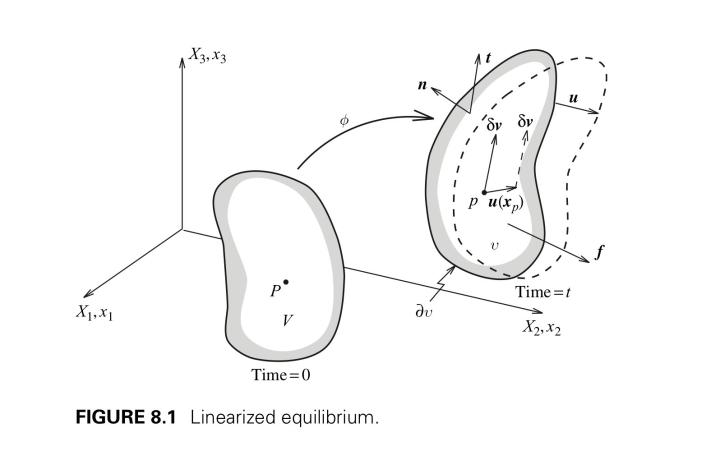
\includegraphics[width=0.5\linewidth]{Figure/fig11}
		\end{figure}
		\begin{itemize}
			\item As shown in the figure, the virtual displacement/velocity is still the same but now the actual quilibrium configuration is changing
			\item At a trial solution $\phi_k$, the virtual work $\delta W(\phi,\delta v) \neq 0$
			
			\item Therefore $D\delta W(\phi_k,\delta v)[u]$ is the change in $ \delta W$ due to $\phi_k$ change to $\phi_k + u$. 
			
			\item Since $\delta v $ is not changing, therefore it is $r$ or the internal forces that are changing as the solution changes due to u
			
			\item NR therfore makes the internal and external forces in equilibrium by changing the configuration to the equilibrium configuration
			\begin{equation}
				D\delta W(\phi, \delta v)[u] = D\delta W_{int}(\phi,\delta v)[u] - D \delta W_{ext}(\phi,\delta v)[u]
			\end{equation}
			\begin{equation}
			D\delta W(\phi, \delta v)[u] = D \left(\int_v \sigma : \delta d~ dv  \right)[u] - D \left( \int_{\Gamma} t.\delta v ~da \right)[u]
			\end{equation}			
		\end{itemize}
	\end{frame}


	\begin{frame}{Lagrangian linearised internal virtual work}
		\begin{itemize}
			\item Linearisation of the equilibrium equations with respect to the material description
			\item Simpler as we have the material description , and we know the dV integral to integrate over
			\item We can push forward the equations to the spatial description
			
			
		\end{itemize}
	\end{frame}

	\begin{frame}{Lagrangian linearised internal virtual work}
		\begin{itemize}
			\item Internal virtual work is given as
			\begin{equation}
				\delta W_{int}(\phi,\delta v) = \int_V S:\dot{\delta E} dV
			\end{equation}
			\item Using product rule for directional derivatives, we get 
			\begin{equation}
				\begin{aligned}
				D 	\delta W_{int}(\phi,\delta v)[u] = D\left(\int_V S:\dot{\delta E} \right)[u] dV\\ 
				\left(\int_V D S:\dot{\delta E} \right)[u] dV\\
     			 \left(\int_V \dot{\delta E} :D S[u] \right) dV + \left(\int_V  S:D \dot{\delta E}[u] \right) dV\\
     			 \left(\int_V \dot{\delta E} :C:D S[u] \right) dV + \left(\int_V  S:D \dot{\delta E}[u] \right) dV\\
				\end{aligned}
			\end{equation}
			(Have to check why can we take the derivative inside the integral?????????????/)		
			\item Where we can then find $D \dot{E}[u]$ Bonet
		\end{itemize}
	\end{frame}


	\begin{frame}
		\begin{itemize}
			\item $D \dot{\delta E}[u]$ is a function of $\delta v$ and also of configuration $\phi$
			\begin{equation}
			\dot{\delta E} = \frac{1}{2}\left(\delta \dot{F}^TF + F^T \delta \dot{F} \right)
			\end{equation}
			and $\delta \dot{F} = \frac{\partial \delta v}{\partial X} = \nabla_o \delta v$ and $DF[u] = \nabla_o u$
			\item So 	
			\begin{equation}
			D\dot{\delta E}[u] = \frac{1}{2}\left(\nabla(\delta v)^T\nabla_ou + \nabla(\delta u)^T\nabla_ov \right)
			\end{equation}
			Here $\nabla_o v$ remains constant, as they are not functions of the configuration
			
		\end{itemize}
	\begin{block}{}
		\begin{equation}
			D\delta W_{int}(\phi,\delta v)[u] = \int_V \dot{\delta E} : C : D E[u] dV + \int_V S : [\left(\nabla_o u \right)^T \nabla_o \delta v] dV 
		\end{equation}
		and $\delta \dot{E}$ can be written as $D E[\delta v]$ which gives a symmetric form:
		\begin{equation}
		D\delta W_{int}(\phi,\delta v)[u] = \int_V {D E[\delta v]} : C : D E[u] dV + \int_V S : [\left(\nabla_o u \right)^T \nabla_o \delta v] dV 
		\end{equation}		
		
	\end{block}
	\end{frame}

	\begin{frame}{Eulerian linearisation}
		\begin{itemize}
			\item The formulations are pushed forward, check Bonet page 219
			
		\end{itemize}
	\end{frame}

	\begin{frame}{Linearised external virtual work}
		\begin{itemize}
			\item Body forces
			\item Surface forces			
		\end{itemize}
	\end{frame}

	\begin{frame}{Variational methods and incompressibility}
	\begin{itemize}
			\item 	The advantage of finding a stationary problem with respect to displacements, is the advantage that such a treatment gives a uniform framework to find
				\begin{itemize}
					\item Incompressibility, contact boundary conditions and finite element methods
					\item Done by use of lagrangian multipliers or penalty methods where the variational principle incorporates eg internal pressure
				\end{itemize}
	\end{itemize}
	\end{frame}

	\begin{frame}{Total potential energy and equilibrium}
		\begin{itemize}
			\item The potential energy whose directional derivative gives the virtual work is
			\begin{equation}
				\Pi(\phi) = \int_V \Psi(C) dV - \int_V f_o. \phi dV - \int_{\Gamma_o} t.\phi dA
			\end{equation}
			\item Assuming that the body force and traction not a function of $\phi$ (Not actuall for traction). The directional derivative is
			\begin{equation}
			\begin{aligned}
			\Pi(\phi)[\delta v] = \int_V S : DC[\delta v]dV - \int_V f_o. \delta v dV - \int_{\Gamma_o} t.\delta vdA
			\end{aligned}
			\end{equation}
			which is similar to the theory of virtual work that is $D\Pi(\phi)[\delta v] = \delta W(\phi,\delta v)$
		\end{itemize}
		\begin{block}{}
			\begin{itemize}
				\item The stationary conition of $\Pi(\phi)$ gives the equilibirum and known as the varitational statement of equilibrium. The lienarised equation (NR) can be taken as the second derivative of the energy functional
				\begin{equation}
					D\delta W(\phi,\delta v)[u] = D^2 \Pi(\phi)[\delta v, u]
				\end{equation}
				\end{itemize}
		\end{block}
	\end{frame}

	\begin{frame}{Incompressibility : Lagrange multiplier}
		\begin{itemize}
			\item We need to keep a incompressibility constraint J =1
			\item Lagrange multiplier term
			\begin{equation}
				\Pi_L(\phi,p) = \hat{\Pi}(\phi) + \int_V p(J-1) dV
			\end{equation}
			where $p$ is the lagrange multiplier with knowing that it will be the internal pressure. $\hat{\Pi}$ is the strain energy given as a function of the distrotion component of the right Cauchy tensor
			\item We will obviously have to find $\Pi_L(\phi,p)[\delta v ]$ and $\Pi_L(\phi,p)\delta p$
			\item And linearise the equilibirum equations again with respect to p and u
			\item Check bonet page 226 for details
		\end{itemize}
	\end{frame}


	\begin{frame}{Incompressibility : Penalty methods}
		\begin{itemize}
			\item Different alternative to Lagrangian methods
			\begin{itemize}
				\item Eliminates pressure as an independant variable keeping a large value of the bulk modulus
				\item Perturb the lagrangian functional with a penalty allowing the pressure to be associated with the deformation
				\begin{itemize}
					\item The perturbed lagrangian is 
					\begin{equation}
						\Pi_P(\phi,p) = \Pi_L(\phi,p) - \int_V \frac{1}{2k}p^2 dV
					\end{equation}
					as $k \rightarrow \infty : \Pi_P \rightarrow \Pi_L$ \\
					with the stationary condition as :
					\begin{equation}
					D\Pi_P(\phi,p)[\delta p] = \int_V \delta p \left((J-1)-\frac{p}{k} \right)dV = 0
					\end{equation}
					The (J-1) comes from the $\Pi_L$ term. Now this euilibrium equation gives us a relationship between p and J as p = k(J-1).
					\item This represents a nearly incompresible material with he penalty number as the bulk modulus (So same thing like increasing bulk modulus)
				\end{itemize}
				
			\end{itemize}
			
		\end{itemize}
	\end{frame}


	\begin{frame}{Hu washizu principle}
		Check bonet page 229
	\end{frame}

	
	\begin{frame}{Mean dilation procedure}
		content
	\end{frame}

\end{document}